\documentclass[10pt,twocolumn,letterpaper]{article}

\usepackage{cvpr}
\usepackage{times}
\usepackage{epsfig}
\usepackage{graphicx}
\usepackage{amsmath}
\usepackage{amssymb}
\usepackage{booktabs}
\usepackage{subcaption}

\def\tightlist{}

% Include other packages here, before hyperref.

% If you comment hyperref and then uncomment it, you should delete
% egpaper.aux before re-running latex.  (Or just hit 'q' on the first latex
% run, let it finish, and you should be clear).
\usepackage[pagebackref=true,breaklinks=true,letterpaper=true,colorlinks,bookmarks=false]{hyperref}

\cvprfinalcopy % *** Uncomment this line for the final submission

\def\cvprPaperID{****} % *** Enter the CVPR Paper ID here
\def\httilde{\mbox{\tt\raisebox{-.5ex}{\symbol{126}}}}

% Pages are numbered in submission mode, and unnumbered in camera-ready
\ifcvprfinal\pagestyle{empty}\fi
\begin{document}

%%%%%%%%% TITLE
\title{Lossy Compression for Machine Perception}

\author{Natalia Frumkin\\
The University of Texas at Austin\\
{\tt\small nfrumkin@utexas.edu}
% For a paper whose authors are all at the same institution,
% omit the following lines up until the closing ``}''.
% Additional authors and addresses can be added with ``\and'',
% just like the second author.
% To save space, use either the email address or home page, not both
\and
Dan Jacobellis\\
The University of Texas at Austin\\
{\tt\small danjacobellis@utexas.edu}
}

\maketitle

%%%%%%%%% BODY TEXT

\begin{abstract}
In the field of neural data compression, the prevailing focus has been on optimizing algorithms for either classical distortion metrics, such as PSNR or SSIM, or human perceptual quality. With increasing amounts of data consumed by machines rather than humans, a new paradigm of machine-oriented compression has emerged, creating several new challenges to the development, evaluation, and deployment of systems utilizing lossy compression. In particular, it is unclear how different approaches to lossy compression will affect the performance of downstream machine perception tasks. To address this under-explored area, we evaluate various perception models—including image classification, image segmentation, speech recognition, and music source separation—under severe lossy compression. We utilize several popular codecs spanning conventional, neural, and generative compression architectures. Our results indicate three key findings: (1) machine perceptual quality correlates strongly with deep similarity metrics; (2) minimal loss in machine perceptual quality can be achieved with very high compression rates; and (3) using lossy compressed datasets, (e.g. ImageNet) for pre-training can lead to scenarios where lossy compression increases machine perceptual quality rather than degrading it. These insights lead us to a novel architecture where intermediate representations learnt from a self-supervised vision model and representation from a reconstruction-trained neural codec are jointly compressed. Our code and experiments are available at: \url{https://github.com/danjacobellis/MPQ}.
\end{abstract}


\begin{figure*}
\begin{center}
\epsfig{width=6.0in,file=Figures/image_compression_methods}
\end{center}
\caption{\label{fig:image_compression_methods}%
Visual comparison of image compression methods. Best viewed zoomed in.}
\end{figure*}


\section{Introduction}

In contemporary machine perception pipelines ~\cite{ehrlich2022first}, lossy compression techniques are often employed, but using legacy codecs at near-lossless quality levels, thus limiting potential savings in data rate. For instance, the ImageNet dataset, a cornerstone for image classification tasks, utilizes JPEG compression with an average compression ratio of roughly 5:1. As a result, the full ImageNet-21k is over 1.3 TB in size, and common practice is to discard most of this information using a 224x224 reduced resolution version~\cite{ridnikimagenet}. Additionally, many types of sensors necessitate extremely high compression ratios, sometimes exceeding 1000:1~\cite{cocker2022low}, resulting from high resolution measurements combined with limited communication bandwidth.

In the decades since the introduction of the ubiquitous JPEG and MPEG standards for images and audio, advancements in lossy compression technologies have demonstrated the capability to achieve far higher compression ratios with less degradation in quality. For example, it has been shown that storing the ImageNet1-1k dataset using the tokens produced by a ViT-VQGAN neural compression model saves a factor of 100:1 in storage and leads to faster and simplified training ~\cite{yu2021vector}\cite{park2023storage}. 
While the advantages of employing more potent lossy compression techniques are evident, uncertainty surrounding their impact on downstream machine perception tasks remains a significant barrier. For example, Ilyas et al ~\cite{ilyas2019adversarial} demonstrate the existence of signal components, called non-robust features, which which are highly predictive yet imperceptible to humans. Lossy compression during training could eliminate these features and lead to sub-optimal models. Additionally, failure to match the exact lossy compression method and settings during training and inference could lead to distribution shift and unpredictable model behavior.

Our work aims to systematically evaluate the impact of various types of lossy compression---both conventional and neural---on both audio and visual machine learning tasks. By addressing these issues, we aim to bridge the gap between the promising capabilities of advanced lossy compression techniques and their practical implementation in machine learning pipelines.

\begin{table}[ht]
\centering
\caption{Summary of Datasets and Models}
\label{tab:datasets_models}
\begin{tabular}{llll}
\toprule
Dataset & Task Type & Model & Metric \\
\midrule
ImageNet-1k & Classification & ViT &  Acc. \\
ChestX-ray8 & Classification & ViT & Acc. \\
Bean Disease & Classification & ViT & Acc. \\
ADE20k & Segmentation & SegFormer & mIOU \\
Common Voice & Recognition & Whisper & WRA \\
MUSDB-HQ & Separation & Demucs v3 & SDR \\
\bottomrule
\end{tabular}
\end{table}

\begin{table}[ht]
\centering
\caption{Summary of Compression Methods}
\label{tab:compression_methods}
\begin{tabular}{lll}
\toprule
Method & Description & Setting \\
\midrule
JPEG & DCT-based coding & Quality: 5 \\
WEBP & Transform coding & Quality: 0 \\
MBT2018 & Neural compression & Quality: 1 \\
HiFiC & Generative compression & Quality: Low \\
MP3 & Audio coding & Bitrate: 8 kbps \\
Opus & Audio compression & Bitrate: 6 kbps \\
EnCodec & Neural audio compression & Bitrate: 6 kbps \\
\bottomrule
\end{tabular}
\end{table}


\section{Methods}

Our study probes the effects of audio and image compression techniques on machine perceptual quality under severe lossy compression. We use six datasets and test the efficacy of popular pre-trained models on various discriminative tasks. Machine perceptual quality is gauged by the performance on the validation splits of these datasets, and the compression performance is evaluated using conventional rate-distortion metrics as well as deep similarity metrics.

We employ the ImageNet-1k dataset for image classification, using a vision transformer (ViT) \cite{dosovitskiy2020image} pretrained on ImagNet-21k . The NIH ChestX-ray8 dataset \cite{wang2017chestx} for pneumonia classification and the bean disease dataset \footnote{\href{https://github.com/AI-Lab-Makerere/ibean}{ibean:Bean disease dataset}} are also used in conjunction with an ImageNet-21k pre-trained ViT. Semantic segmentation is performed on the ADE20k dataset \cite{zhou2017scene} using the SegFormer model \cite{xie2021segformer}. The Common Voice 11.0 dataset \cite{ardila2020common} and the Whisper model \cite{radford2023robust} are used for speech recognition. Finally, the MUSDB-HQ dataset, an uncompressed version of MUSDB18 \cite{rafii2017musdb18}, and the Demucs v3 model \cite{defossez2021hybrid} are used for music source separation. These datasets and corresponding models are summarized in \ref{tab:datasets_models}.

The compression methods in our study encompass JPEG, WEBP, the neural compression approach Minnen, Ballé, Toderici 2018 (mbt2018) \cite{minnen2018joint} as implemented in Compressai \cite{begaint2020compressai}, HiFiC \cite{mentzer2020high} from the Tensorflow Compression library \cite{balle2022tensorflow}, the audio codecs MPEG Layer III (MP3), Opus, and the neural audio model EnCodec \cite{defossez2022high}. Table \ref{tab:compression_methods} summarizes these methods.

To evaluate compression performance, we include conventional rate-distortion figures alongside two deep similarity metrics: Learned Perceptual Image Patch Similarity (LPIPS) \cite{zhang2018unreasonable} for images and Contrastive Deep Perceptual Audio Similarity Metric (CDPAM) \cite{manocha2021cdpam} for audio. These metrics are computed per sample and averaged over the entire dataset.

\begin{table*}
\centering
\caption{Feature Compression Results using BeiT-2}
\label{tab:feature_compression_results}
\begin{tabular}{lccccc}
\toprule
Downstream Task & Compression Scheme & Finetune All & Finetune Task Layer Only & BPP & Compression Ratio \\
\midrule
% \multicolumn{5}{c}{BeiT Image Classification} \\
\cmidrule(lr){1-5}
& None & 86.4 & 86.2 & 0.490 & 49 \\
BeiT Image Classification  & with 8-bit FSQ & \textbf{87.7} & \textbf{87.7} & 0.041 & 588 \\
&INT8 Quantized Code & 86.4 & 86.1 & 0.122 & 196 \\
&INT2 Quantized Code & 85.4 & 85.2 & \textbf{0.031} & \textbf{784} \\
\midrule
% \multicolumn{5}{c}{BeiT Semantic Segmentation} \\
\cmidrule(lr){1-5}
BeiT Semantic Segmentation & None & \textbf{53.5} & 53.0 & 2006 & 0.0120 \\
 % & with 32-bit FSQ & - & 52.18 & 128 & 0.1875 \\
 & with 8-bit FSQ & - & 41.65 & 32 & 0.75 \\
  & add all features & - & 54.74 & 32 & 0.75 \\
\bottomrule
\end{tabular}
\end{table*}

\textbf{Feature Compression Approach}.
Due to the inherent limits of full-input machine-oriented compression, we investigate an alternative architecture based on feature compression. We compute the embeddings produced by BeiT-2, a self-supervised vision transformer that is known to generate representations that transfer effectively to a variety of tasks, including image classification and segmentation \cite{peng2022beit}. While these representation are known to be effective for downstream tasks, they are considerably larger than the corresponding compressed image. To mitigate this, we explore the training of a neural compression model specifically tailored to these high-dimensional features \cite{singh2020end}. Our codec is based on Finite Scalar Quantization (FSQ), a simplified variant of the VQ-VAE. \cite{mentzer2023finite}.

\begin{figure*}
\begin{center}
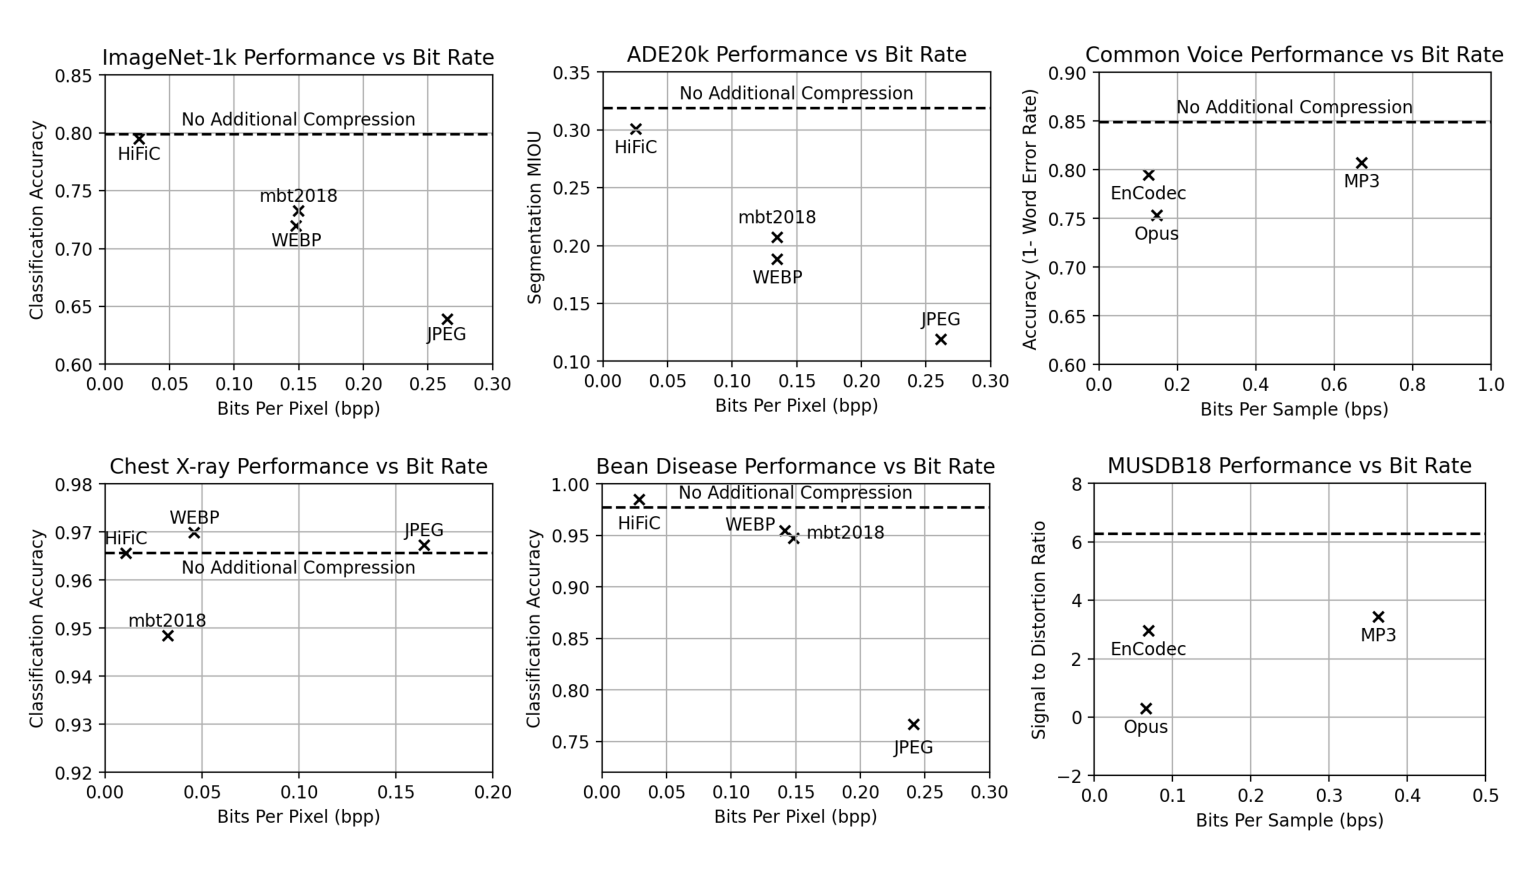
\epsfig{width=6.0in,file=Figures/mpq_results}
\end{center}
\caption{\label{fig:example}%
Performance on various machine perception tasks under full-input machine coding.}
\end{figure*}

\begin{table*}[!htb]
    \caption{Comparing Compression \& Machine Perceptual Quality across Various Techniques}
    \label{tab:compression_comparison}
        \begin{subtable}{.6\linewidth}
      \centering
        \caption{Summary of Image Results}
        \label{tab:image_compression_comparison}
        \setlength{\tabcolsep}{3pt}
        {\small\begin{tabular}{lcccccc}
\toprule
Metric & Dataset & Baseline & JPEG & WEBP & MBT & HiFiC \\
\midrule
     & ADE20k &  & 23.9 & 25.6 & \textbf{28.1} & 27.7 \\
     & Bean &  & 20.8 & 22.0 & \textbf{22.9} & 21.8 \\
     & X-ray &  & 30.0 & 32.7 & 34.7 & \textbf{36.4} \\
\midrule
LPIPS & ImageNet &  & 6.11 & 7.02 & 7.95 & \textbf{10.8} \\
      & ADE20k &  & 7.13 & 7.96 & 8.99 & \textbf{11.8 }\\
      & Bean &  & 5.72 & 6.75 & 6.90 & \textbf{9.78} \\
      & X-ray &  & 6.85 & 7.58 & \textbf{7.80} & 13.2 \\
\midrule
BPP & ImageNet &  & \textbf{0.26} & 0.148 & 0.150 & 0.026 \\
    & ADE20k &  & \textbf{0.26} & 0.14 & 0.14 & 0.025 \\
    & Bean &  & 0.24 & 0.14 & 0.15 & \textbf{0.029} \\
    & X-ray &  & \textbf{0.17} & 0.046 & 0.032 & 0.011 \\
\midrule
Top-1 & ImageNet & \textbf{0.799} & 0.639 & 0.720 & 0.733 & 0.795 \\
 Accuracy                        & Bean & 0.977 & 0.767 & 0.955 & 0.947 &\textbf{ 0.985} \\
                        & X-ray & 0.966 & 0.967 & \textbf{0.970} & 0.948 & 0.966 \\
\midrule
mIOU & ADE20k & \textbf{0.319} & 0.119 & 0.189 & 0.208 & 0.301 \\
\bottomrule
\end{tabular}}
    \end{subtable} 
    \begin{subtable}{.4\linewidth}
      \centering
        \caption{Summary of Audio Results}
        \label{tab:audio_compression_comparison}
         \setlength{\tabcolsep}{3pt}
        {\small\begin{tabular}{lccccc}
        \toprule
        Metric & Dataset & Baseline & MP3 & OPUS & EnCodec \\
        \midrule
        PSNR & MUSDB18 &  &\textbf{ 29.17} & 22.17 & 24.95 \\
             & CV &  & \textbf{33.89} & 26.70 & 29.04 \\
        \midrule
        CDPAM & MUSDB18 &  & 38.43 & 36.46 & \textbf{45.33} \\
              & CV &  & 37.89 & 38.27 & \textbf{46.34} \\
        \midrule
        BPS & MUSDB18 &  & \textbf{0.36} & 0.066 & 0.069 \\
            & CV &  & \textbf{0.67} & 0.14 & 0.13 \\
        \midrule
        SDR & MUSDB18 & \textbf{6.29} & 3.44 & 0.30 & 2.97 \\
        \midrule
        WRA & CV & \textbf{0.85} & 0.81 & 0.75 & 0.80 \\
        \bottomrule
        \end{tabular}}
    \end{subtable}%
\end{table*}


\section{Results}

Our evaluation across multiple datasets and machine perception tasks reveals key insights into the impact of lossy compression on machine perceptual quality. The results are summarized in Table~\ref{tab:compression_comparison}.
For image-based tasks, LPIPS is a better predictor of downstream performance than PSNR, and generative compression (HiFiC) performs the best at all but one of the tasks (Chest X-ray) despite having the lowest average bitrate, and consistently achieves results close to the uncompressed baseline.
In the audio domain, similar trends are observed; the audio quality measured by CDPAM is better predictor of downstream performance than PSNR, and, among the methods tested, EnCodec provides the best tradeoff between rate and downstream performance for both datasets.

Our initial feature compression experiments demonstrate promising results. As shown in table ~\ref{tab:feature_compression_results}, utilizing FSQ allows us to achieve a high compression rate with no loss in classification accuracy. For semantic segmentation, we are presented with a significant compression challenge -- the encoder generates a large intermediary representation (size is [4,678,32,32]) which leads to a 2,006 bits-per-pixel, however, we plan to consider extreme compression techniques, including FSQ, to attempt at reaching $\sim 0.1$ bits-per-pixel.
\section{Discussion}

\textbf{Deep similarity metrics and generative compression}. It is well known that deep similarity metrics are highly effective at predicting human perceptual quality as measured by mean opinion score (MOS). Across the six datasets tested, our results indicate that these metrics are also strongly correlated with machine perceptual quality, measured by the downstream performance of machine learning models. One may be concerned that generative compression methods (e.g. HiFiC and EnCodec) which discard and re-synthesise details are ill-suited for use within machine perception pipelines. However, our results indicate that this is not the case for any of the tasks tested.

\textbf{Pretraining on lossy datasets}. Our experiments reveal an intriguing phenomenon: for models pre-trained on lossy datasets like ImageNet, additional lossy compression at test time may have negligible impact on performance, and can sometimes behave as an enhancement. For example, the top-1 classification accuracy on the bean disease dataset is higher when compressed using HiFiC (compression ratio of 839:1) than when using the original lossless images. Even more surprising is that JPEG compression (see ~\ref{fig:image_compression_methods}) results in an increase in pneumonia classification performance on the Chest X-ray dataset, despite having the lowest quality measured by PSNR or LPIPS. Viewing lossy compression as a type of distribution shift provides one possible explanation for this phenomenon; subtle high-frequency details that only exist in lossless images never occur in pre-training datasets like the JPEG-compressed ImageNet.

\textbf{Next Steps}
From our BeiT classification experiments, we are successful at generating high compression ratios of $> 100:1$ using FSQ and standard integer quantization. In our next phase of this project, we will address the harder problem of compression for semantic segmentation.

Handling variable-size images \& audio remains a key challenge in machine-oriented compression systems. For example, most image compression techniques automatically resize images to 224x244, which purposefully removes information prior to compression. Our results for feature compression indicate a promising path forward: by maintaining two representations (one fixed in size and another variable) which are jointly compressed, we can maintain good reconstruction quality and near-lossless performance on downstream tasks.

{\small
\bibliographystyle{ieee_fullname}
\bibliography{egbib}
}

\end{document}
